% Autor: Manuel Lippert
% Physikalisches Praktikum

% Main-Datei für die Auswertung in TeX

% Struktur:
% Jedes Kapitel hat einen Input-File. Um Merge-Konflikte zu verhindern wird angeraten für jede 
% Datei eine eigene Tex Datei zu machen und sie im jeweiligen Kapitel zu importieren. Die in
% Input-Struktur dient zur besseren Übersicht und für mögliche Ordner, welche hier vorhanden sind. Die Zahlen vor den 
% Ordner dient zur Ordnung der einzelnen tex-Files nach Kapiteln


% Packages
\documentclass[paper=a4,bibliography=totoc,BCOR=10mm,twoside,numbers=noenddot,fontsize=11pt]{scrreprt}
\usepackage[english]{babel}
\usepackage[T1]{fontenc}
\usepackage[latin1, utf8]{inputenc} %ä, ö, ü inbegriffen
\usepackage[babel,german=quotes]{csquotes} %For Quotes
\usepackage{lmodern}
\usepackage{graphicx}
\usepackage{nicefrac}
\usepackage{fancyvrb}
\usepackage{amsmath,amssymb,amstext}
\usepackage{siunitx}
\usepackage{url}
\usepackage{natbib}
\usepackage{microtype}
\usepackage[format=plain]{caption}
\usepackage{physics}
\usepackage{titleref} 

% Zusätzliche Packages
\usepackage{geometry} % Verändert Seitengeometrie
\usepackage{anyfontsize} % Alle Schriftgrößen möglich machen
\usepackage[table]{xcolor} % Farbliche Gestaltung Tabellen
\usepackage{ifthen} % Für kompliziertere tex-Files
\usepackage[absolute,overlay]{textpos} %Textboxen
\usepackage{amsfonts} % Schriftarten
\usepackage{xstring} % Stringoperationen
\usepackage{tikz} % Zeichnungen
\usepackage{pdfpages} % Import von pdfs (Protokolle)
\usepackage{hyperref} % Verlinkungen im Dokument
\usepackage{makecell} % Zeilenumbruch in Zelle

% Abschnittseinrückung und -abstand
% Die folgenden Zeilen sollen möglichst nicht verändert werden
\parindent 0.0cm
\parskip 0.8ex plus 0.5ex minus 0.5ex

% Anzahl und Größe von Gleitobjekten
% maximal 2 Objekte oben und unten
% erlaubt auch größere Bilder, welche die ganze Seite benötigen
% Die folgenden Zeilen sollen möglichst nicht verändert werden
\setcounter{bottomnumber}{2}
\setcounter{topnumber}{2}
\renewcommand{\bottomfraction}{1.}
\renewcommand{\topfraction}{1.}
\renewcommand{\textfraction}{0.}

%\sc und \bc veraltet. Daher: (20.09.2018)
\DeclareOldFontCommand{\sc}{\normalfont\scshape}{\@nomath\sc}
\DeclareOldFontCommand{\bf}{\normalfont\scshape}{\textbf}

% Verschiedenes
\pagestyle{headings}          % Der Seitenstil sollte möglichst nicht verändert werden
\graphicspath{{./Bilder/}}    % Der Pfad für die Abbildungen Abbildungen wird gesetzt
\VerbatimFootnotes            % \verb etc. auch in \footnotes mφglich

% Funktionen
\newcommand\tab[1][1cm]{\hspace*{#1}}
\newcommand{\vect}[1]{\boldsymbol{\mathbf{#1}}}
\newcolumntype{g}{>{\columncolor[rgb]{ .741,  .843,  .933}}l}
% Tiefgestellte Zahlen nicht kursiv
\catcode`_=\active
\newcommand_[1]{\ensuremath{\sb{\mathrm{#1}}}}

\begin{document}

    \nonfrenchspacing

    % 0.Chapter Cover
    % 0. Cover

% Hier sind nur die Variablen und der Abschnitt Informationen (unten) zu bearbeiten der REst läuft automatisch ab (z.b Farbenänderung)

% Noch abänderbar nur ein Vorschlag
\newgeometry{top=30mm, bottom=20mm, inner=20mm, outer=20mm}
\thispagestyle{empty}

% Colors (Notability Colors)
\definecolor{Notablue}{HTML}{3498DB}		
\definecolor{Notared}{HTML}{CF366C}			
\definecolor{Notagreen}{HTML}{19B092}		
\definecolor{Notaorange}{HTML}{FA9D00}		
\definecolor{Notagrey}{HTML}{969696}		
\definecolor{Notalavendel}{HTML}{9DBBD8}	

% Boolean by default false. Für Absatz in der Überschrift
\newboolean{twoRows}
\newboolean{symbol}

% Funktions
\makeatletter
   \def\vhrulefill#1{\leavevmode\leaders\hrule\@height#1\hfill \kern\z@}
\makeatother
\newcommand*\ruleline[1]{\par\noindent\raisebox{.8ex}{\makebox[\linewidth]{\vhrulefill{\linethickness}\hspace{1ex}\raisebox{-.8ex}{#1}\hspace{1ex}\vhrulefill{\linethickness}}}}

% Variables
\def\schriftgrosse{70}
\def\linethickness{1,5pt}

\def\farbe{black}
\def\fach{PPBphys2}
\def\name{Manuel Lippert - Paul Schwanitz}
\def\titel{Rasterelektronen- \\[0,5cm] mikroskop} % Absatz mit \\[0,5cm]; u = Übung, k = Klausur; s = Skript, e = Ergebnis
\def\bottom{WS2021/22}
\def\datum{13.09.2021}
\def\platz{NWII | 2.1.00.267}
\def\betreuer{Inga Elvers}

\def\teilnehmerm{Manuel Lippert}
\def\emailm{Manuel.Lippert@uni-bayreuth.de}
\def\teilnehmerp{Paul Schwanitz}
\def\emailp{Paul.Schwanitz@uni-bayreuth.de}

%\def\auswertp{}
%\def\messp{}
%\def\protop{}

\def\groupnr{11}

\begin{titlepage}
			
	\centering
	{\LARGE \sffamily {\textbf{\bottom}\par}}
	\vspace{2,5cm}
    {\fontsize{30}{0}\sffamily\ruleline{\textcolor{\farbe}{\textbf{\fach}}}\par}
    \vspace{6cm}
	{\Large\sffamily \ruleline{\name}\par}
		
	\IfSubStr {\titel} {\\[0,5cm]} {\setboolean{twoRows}{true}} {\setboolean{twoRows}{false}}
	
	\ifthenelse{\boolean{twoRows}}
		{
			\begin{textblock*}{21cm}(0cm,8cm) % {block width} (coords), centered		
				{\fontsize{\schriftgrosse}{0}\sffamily\textcolor{\farbe}{\textbf{\titel}}\par}
			\end{textblock*}
		}
		{
			\begin{textblock*}{21cm}(0cm,9cm) % {block width} (coords), centered		
				{\fontsize{\schriftgrosse}{0}\sffamily\textcolor{\farbe}{\textbf{\titel}}\par}
			\end{textblock*} 
		}
	
	% Choose Logo
	\ifthenelse {\equal{\farbe}{Notared}} {\def\logo{Bilder/Logo/UniBTNotared}}
		{\ifthenelse {\equal{\farbe}{Notagreen}} {\def\logo{Bilder/Logo/UniBTNotagreen}}
			{\ifthenelse {\equal{\farbe}{Notablue}} {\def\logo{Bilder/Logo/UniBTNotablue}}
				{\ifthenelse {\equal{\farbe}{Notaorange}} {\def\logo{Bilder/Logo/UniBTNotaorange}}
					{\ifthenelse {\equal{\farbe}{Notagrey}} {\def\logo{Bilder/Logo/UniBTNotagrey}}
						{\ifthenelse {\equal{\farbe}{Notalavendel}} {\def\logo{Bilder/Logo/UniBTNotalavendel}}	
							{\ifthenelse {\equal{\farbe}{black}} {\def\logo{Bilder/Logo/UniBT}}	
								{\def\logo{noLogo}}
							}
						}
					}
				}
			}
		}	

	\IfSubStr{\logo}{noLogo}{\setboolean{symbol}{false}}{\setboolean{symbol}{true}}
	
	% Gruppe
	\vspace{10cm}
	{\large\sffamily{Gruppe \groupnr}}
	
	%Logo
	\vfill

	\ifthenelse{\boolean{symbol}}
		{
			\begin{figure}[h]
			\begin{center}
				
				\includegraphics[width=2cm]{\logo}
				
			\end{center}
			\end{figure}
		}
	
\end{titlepage}

\restoregeometry

% Information
\chapter*{Informationen}
\label{chap:info}

\begin{tabular}{l l}

	{\textbf{Versuchstag}} \hspace{1cm} & \hspace{1cm} {\datum}\\[0,2cm]
	{\textbf{Versuchsplatz}} \hspace{1cm} & \hspace{1cm} {\platz}\\[0,2cm]
	{\textbf{Betreuer}} \hspace{1cm} & \hspace{1cm} {\betreuer}\\[1,2cm]
	{\textbf{Gruppen Nr.}} \hspace{1cm} & \hspace{1cm} {\groupnr}\\[0.2cm]
	% Für Fortgeschittenenen Praktikum
	{\textbf{Teilnehmer}} \hspace{1cm} & \hspace{1cm} {\teilnehmerm~(\emailm)}\\[0.2cm]
						  \hspace{1cm} & \hspace{1cm} {\teilnehmerp~(\emailp)}\\[0.2cm]
	% Für Grundpraktikum
	%{\textbf{Auswertperson}} \hspace{1cm} & \hspace{1cm} {\auswertp}\\[0.2cm]
	%{\textbf{Messperson}} \hspace{1cm} & \hspace{1cm} {\messp}\\[0.2cm]
	%{\textbf{Protokollperson}} \hspace{1cm} & \hspace{1cm} {\protop}\\[0.2cm]

\end{tabular}

    \thispagestyle{empty}
    \cleardoublepage
    \tableofcontents
    \cleardoublepage

    % 1.Chapter Instructions
    % 1. Introduction

\chapter{Introduction}
\label{chap:intro}

% Text

    % 2.Chapter Theorie
    \chapter{Theoretical background}

\section{Saturation spectroscopy in general}
With saturation spectroscopy enables us to see the hyperfine structure, because with this methode it is theoretical possible to bypass the dopplereffect. \\
By saturation spectroscopy a laser (pump beam) beam will pass a gas sample (with doppler widened absorption transitions). That caused a stimulation of specific atoms, depending from there speed. 

Vice versa to the pump beam another laser beam with the same frequency (probe beam) will also pass the gas sample.

If now a photon is absorbed, the atom must have a speed component ($v_z$ parallel to the laser beams) in the intervall: 
\begin{align}
    v_{\text{z}} \pm \Delta v_{\text{z}} = \frac{\omega -\omega_0 \pm \delta \omega_{\text{n}}}{k}
\end{align}
In this connection: 
\begin{itemize} 
    \item $\delta \omega_{\text{n}}$ is the homogeneous line width.
    \item $\Delta v_{\text{z}}$ is the width of the hole in the occupation distribution.
    \item $\omega$ is the frequency of the laser.
    \item $\omega_0$ is the resonance frequency of the wanted transition.
    \item $k$ 
\end{itemize}

Because many atoms are stimulated, the probe beam hits barley atoms that can be stimulated. For this reason we obtain the occupation distribution $N(v_{\text{z}})$ and the adsorption profile $\alpha(\omega)$. For this experiment the laser frequency is so chosen, that the fit with the resonance frequency of the wanted transition \citep{VA}.

\section{Preparatory questions}

\paragraph{1. Nuclear spin}
Because the isotopes have a different nuclear structure and the spin depends on that structure, the spins are different. Below the quantum numbers of the basic condition and the fist two stimulated conditions: 
\begin{table}[h]
    \centering
    \begin{tabular}{|c|c|c|c|c|}
        \hline
        Element Name & basic condition & first stimulated condition & second stimulated condition \\
        \hline\hline
        Rb-85 & $5^2$S$_{\frac{1}{2}}$ $\Rightarrow$ F = 2, 3 & $5^2$P$_{\frac{1}{2}}$ $\Rightarrow$ F = 2, 3 & $5^2$S$_{\frac{3}{2}}$ $\Rightarrow$ F = 1, 2, 3, 4 \\
        \hline
        Rb-87 & $5^2$S$_{\frac{1}{2}}$ $\Rightarrow$ F = 1, 2 & $5^2$P$_{\frac{1}{2}}$ $\Rightarrow$ F = 1, 2 & $5^2$S$_{\frac{3}{2}}$ $\Rightarrow$ F = 0, 1, 2, 3 \\
        \hline
    \end{tabular}
    \caption{Quantum numbers of Rb-85 and Rb-87}
\end{table}

\newpage
\paragraph{2. Importent terms}

\subparagraph{Natural line width}

\subparagraph{Doppler broadening}

\subparagraph{Homogeneous/inhomogeneous widening}

\subparagraph{Saturation widening}


\paragraph{3. Cross-over resonances}


\paragraph{4. Beam splitter and $\lambda$/2 plate}


\paragraph{5. Hyperfine structure}

    % 3.Kapitel Protocol
    % 3. Protocol

\chapter{Protocol}
\label{chap:protocol}

\section*{Adjustment for measurement}
We adjust the test setup after instruction of the supervisor with the adjusting tip. For that we make sure to take two points for two mirrors that are as far as possible away from the specific mirror.

\section*{Chanels}

\begin{tabular}[]{c|c|l}
    Input & Output & Description\\
    \hline
    ai0 & RF Output & balance of reference beam and measurement beam\\
    ai1 & Monitor + & measurement beam\\
    ai3 & Monitor - & reference beam\\
    ai4 & PD2 Output & signal of fabry-pérot-interferometer\\
\end{tabular}\\

For our files we have taken the name: \textit{MesN\_TempY\_ZPeaks} there $N$ is number of the measurement/id and $Y$ is the temperature \SI{24}{\celsius}, \SI{38}{\celsius}, \SI{56,2}{\celsius} without the unit and $Z$ is the number to identify the peak with the values all, 1, 2, 3, 4 which is number from left to right.
To every measurement we save a .dat-file and a .bmp-file on our usb-stick.
We also used always the act-value and not the set-value for measurement.

\section*{Measurement}
\begin{itemize}
    \item \textbf{Temperature: \SI{24}{\celsius}} \\ 
    Filename: \textit{date+time\_group11\_MesN\_Temp24\_ZPeak.dat and .bmp}\\ $N$ from 1 to 5, act-value: \SI{24}{\celsius}
    \item \textbf{Temperature: \SI{38}{\celsius}} \\ 
    Filename: \textit{date+time\_group11\_MesN\_Temp38\_ZPeak.dat and .bmp}\\ $N$ from 6 to 10, act-value: \SI{40}{\celsius}
    \item \textbf{Temperature: \SI{56,2}{\celsius}} \\ 
    Filename: \textit{date+time\_group11\_MesN\_Temp38\_ZPeak.dat and .bmp}\\ $N$ from 11 to 15, act-value: \SI{60}{\celsius}
    \item \textbf{Distance fabry-pérot-interferometer:} \SI{72,5}{\centi\metre}+\SI{36}{\centi\metre}+\SI{43}{\centi\metre}=\SI{151,5}{\centi\metre}\\ measured with tape measure
\end{itemize}

\begin{center}
    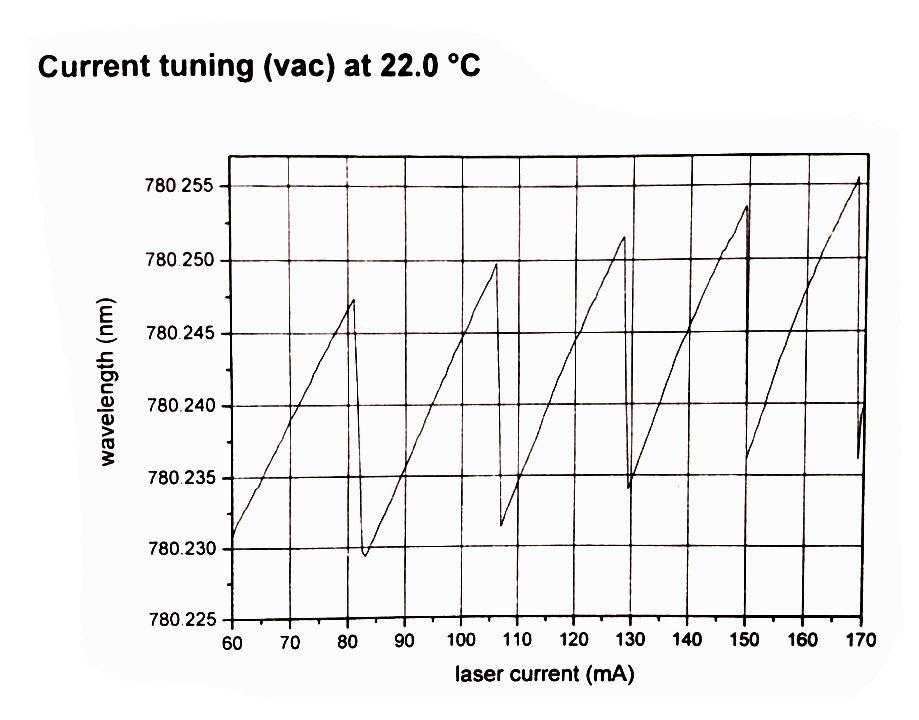
\includegraphics[scale = 0.4]{currentTuning.jpg}
    \captionof{figure}{Currunt Tuning at \SI{22}{\celsius} from laser instructions}
    \label{image:currentTuning}
\end{center}

    % 4.Kapitel Evaluation
    % 4. Evaluation

\chapter{Evaluation}
\label{chap:eval}

% Text

% Part 1

\section{Freeing Absorption Spectrum from Trend and identify Lines}
\label{sec:freeing}
Now we want to free the spectrum from any trend for that the fit a linear function on the spectrum of the reference beam and subtract the fit from the sample beam and reference beam. It is worth mentioning that we have moved the reference beam spectrum down to the niveau of the sample beam spectrum and after that we fitted the linear function. In fig. \ref{image:trends} we can see the absorption spectrum with trends and the linear fit and in fig. \ref{image:trendless} the spectrum without trends. The fit is managed with the function polyfit of the numpy-module in python. We did also cut the data so that we can clearly see the four peaks without any jumps in mode.
\begin{center}
    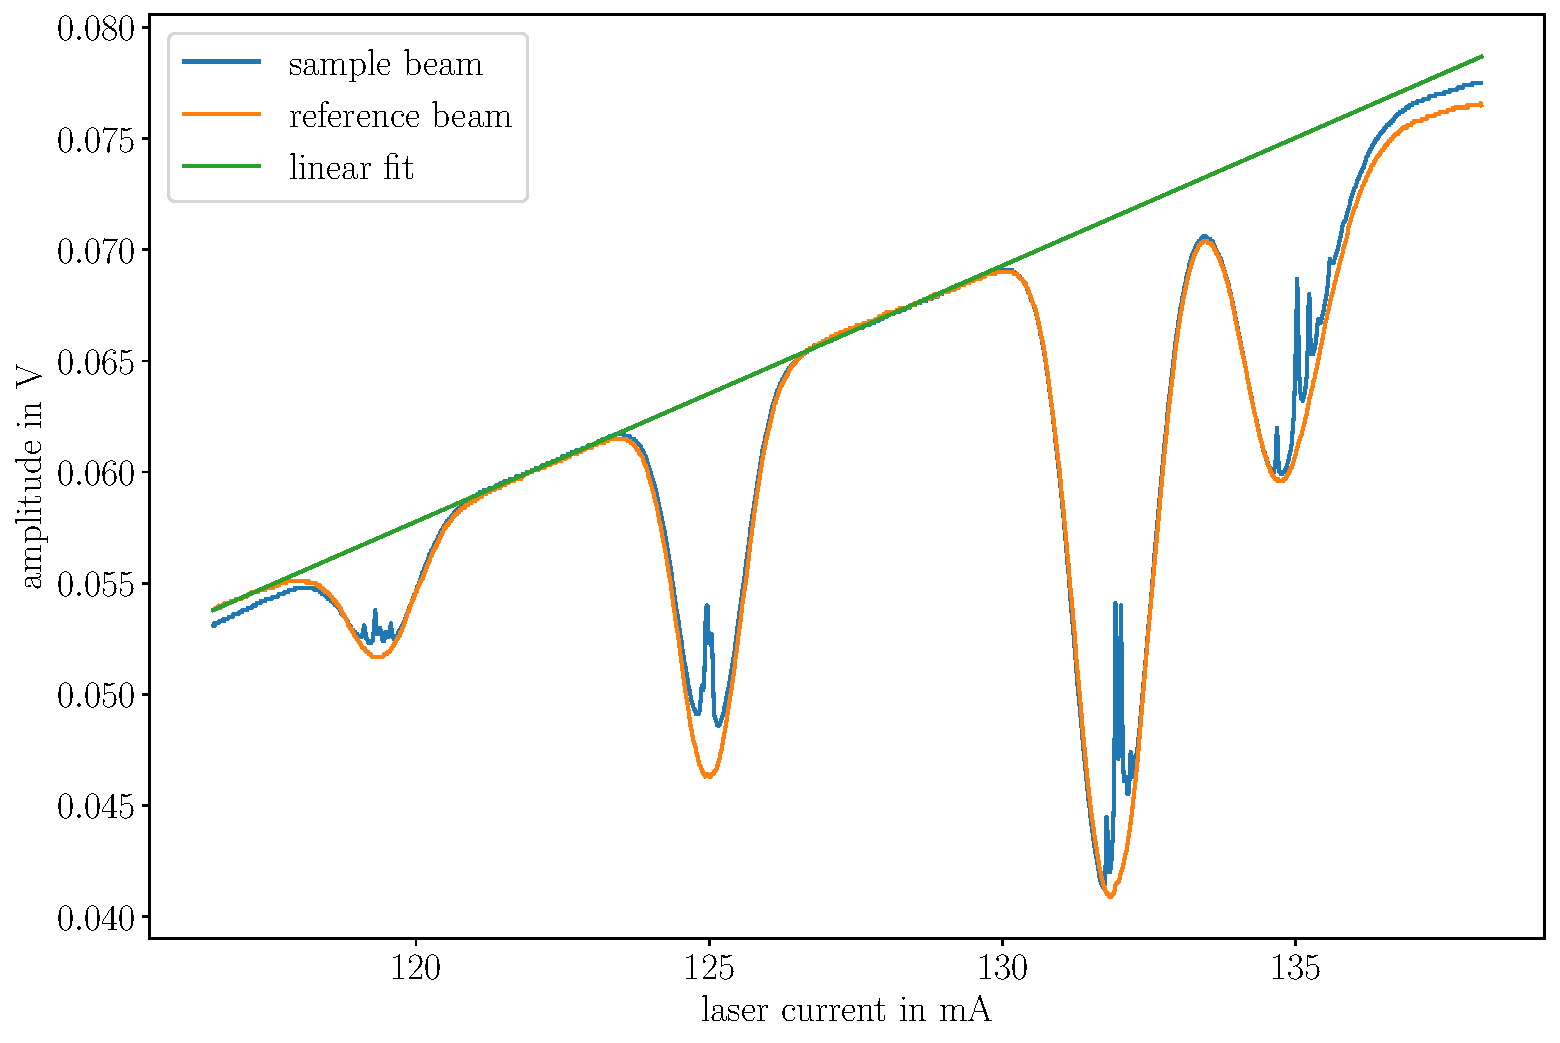
\includegraphics[scale=0.47]{Aufg-1/trend24.pdf}
    \captionof{figure}{absorption spectrum with trends}
    \label{image:trends}
\end{center}
\begin{center}
    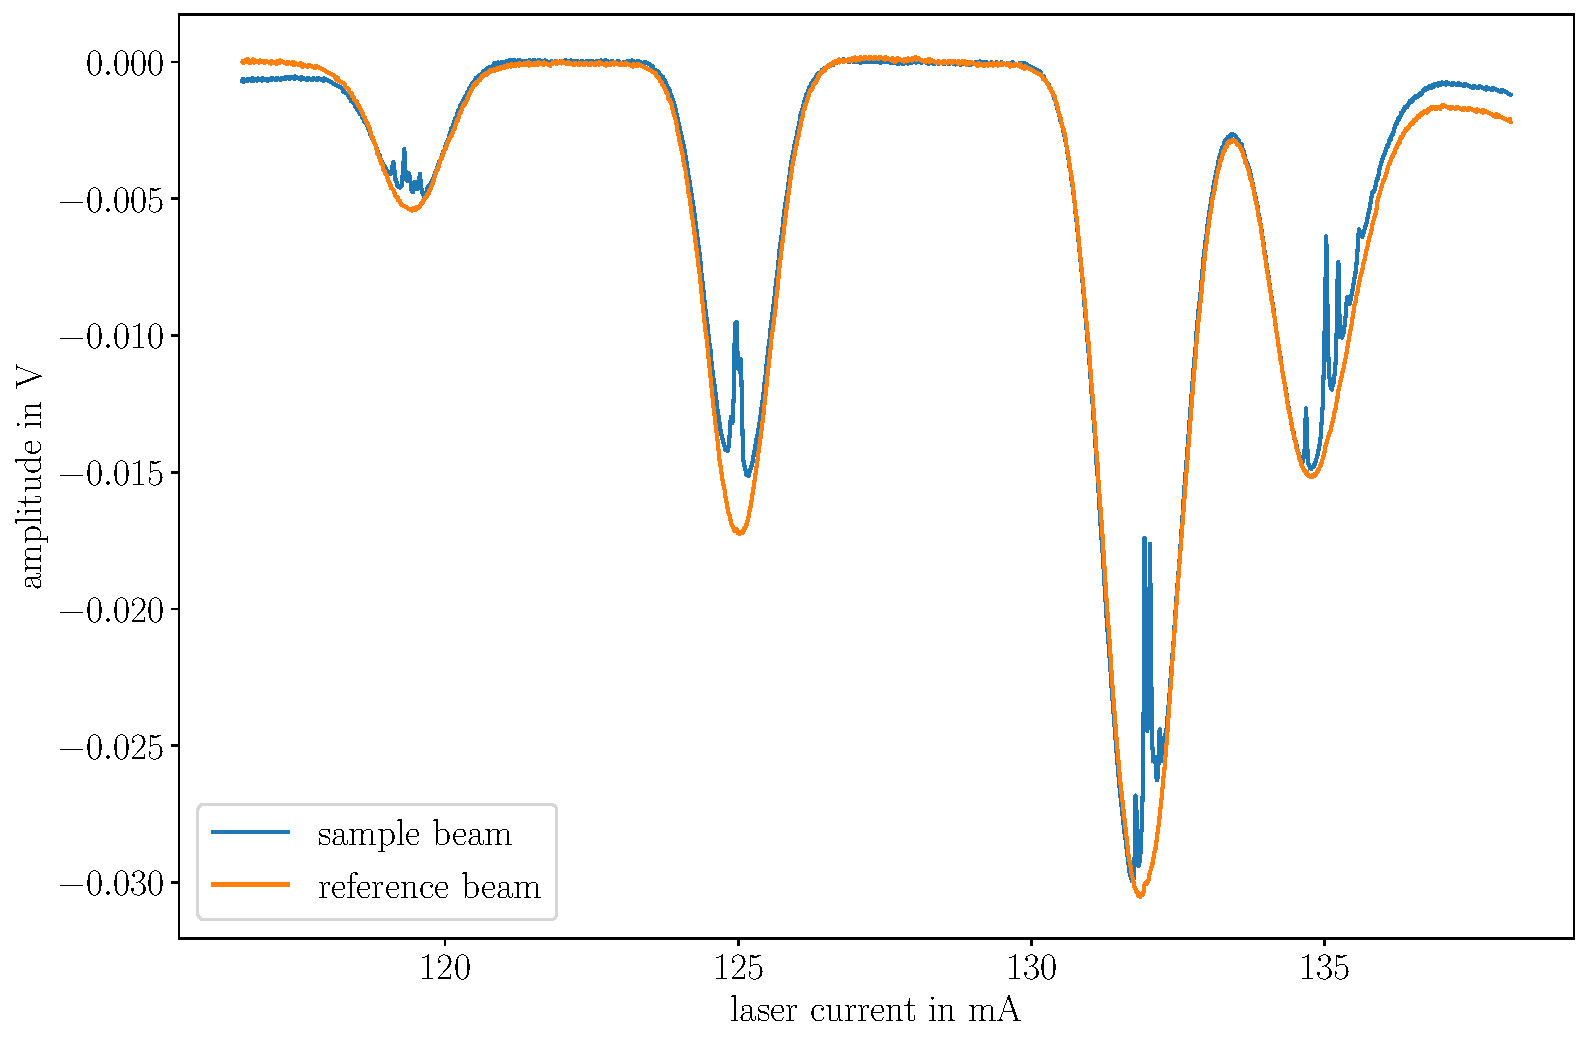
\includegraphics[scale=0.47]{Aufg-1/trendless24.pdf}
    \captionof{figure}{absorption Spectrum without trends}
    \label{image:trendless}
\end{center}
We applied the same procedure on the data of the fabry-pérot and see clear in fig. \ref{image:allTrendless} that the signal is not very stable, but this is not from interest for the upcoming evaluation because we need only the distance between to peaks.
\begin{center}
    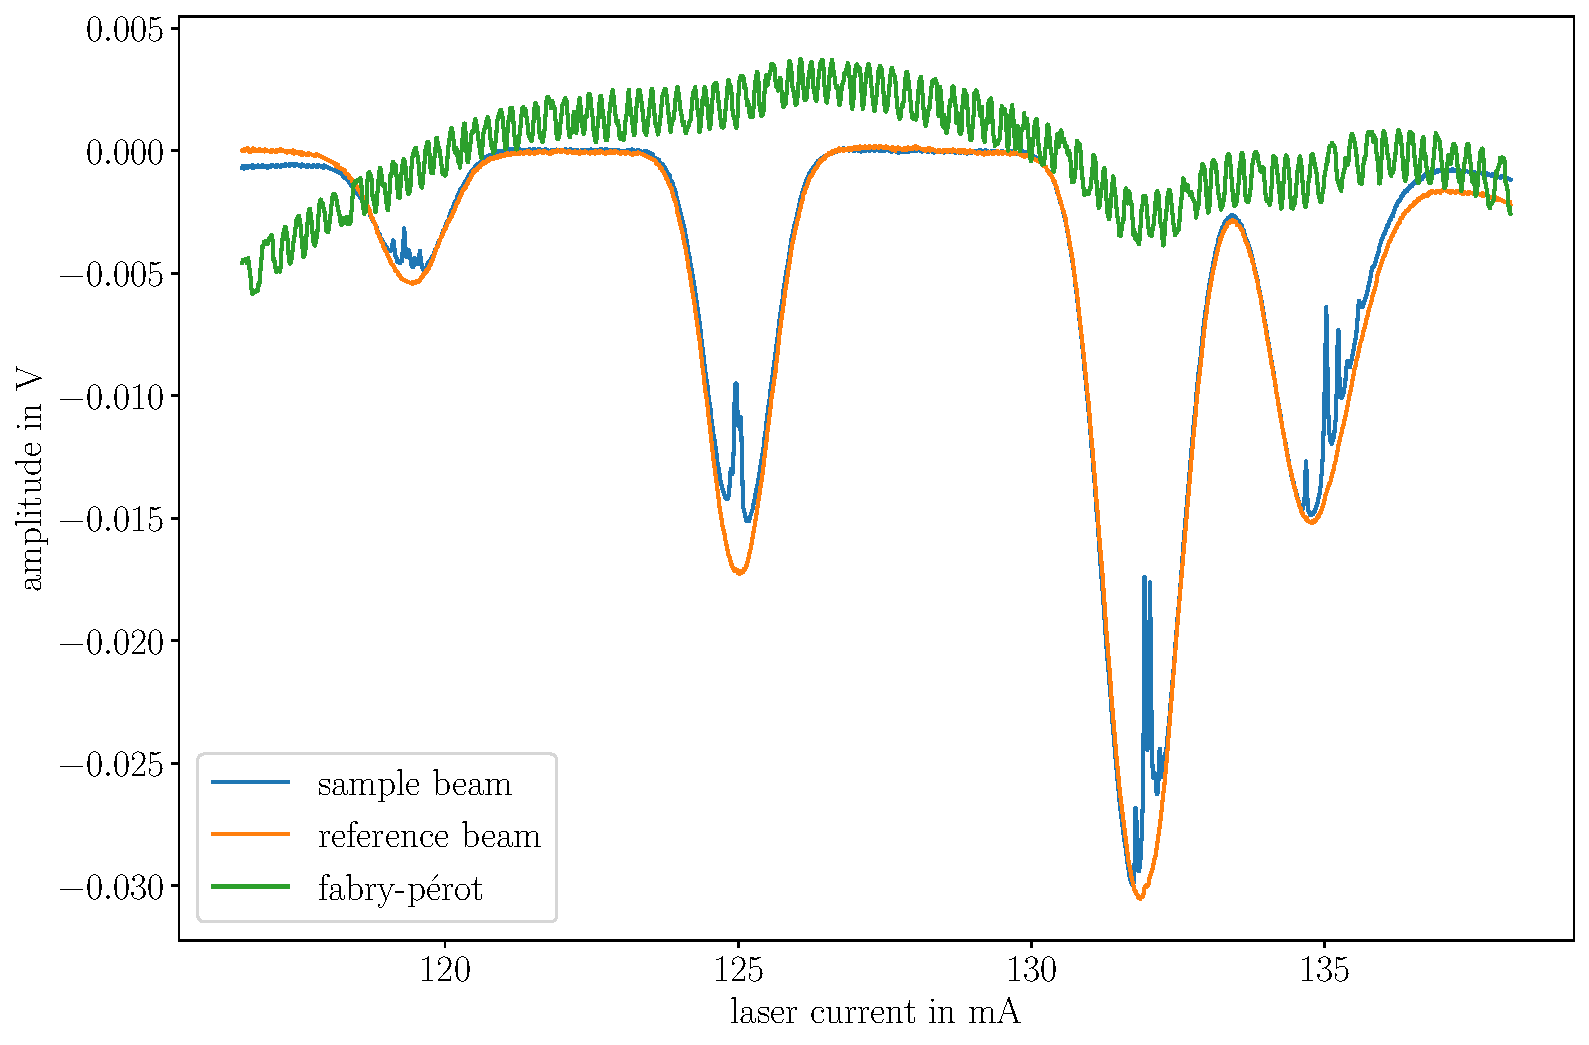
\includegraphics[scale=0.47]{Aufg-1/alltrendless24.pdf}
    \captionof{figure}{absorption spectrum without trends all channels}
    \label{image:allTrendless}
\end{center}
\subsection*{Identfication considering intensity and order}
To identify the lines of the spectrum we used the current wavelength curve (look fig. \ref{image:currentTuning}) to convert the laser current to the wavelength. To do this we convert the fig. \ref{image:currentTuning} into a csv-file using python. For that we measured roughly the points of the peaks from 105 mA to 150 mA (because that is the area of interest) and calculated a basic linear function of the form $y=mx +t$ between them (look fig. \ref{image:currentTuningCut}). Then we obtain three separate linear functions that can transform our data in the corresponding wavelength in the specific area of the current wavelength curve.
\begin{center}
    \begin{tabular}{c | c c c c}
        {} & 1 & 2 & 3 & 4 \\
        \hline
        laser current/mA & 107.0 & 128.5 & 129.5 & 149.5\\
        wavelength/nm & 780.23125 & 780.25125 & 780.234 & 780.2535\\
    \end{tabular}
    \captionof{table}{point used for recreating current wavelength curve}
    \begin{tabular}{c | r r }
        area & m/$\frac{\text{nm}}{\text{mA}}$ & t/nm\\
        \hline
        $1 \rightarrow 2$ & 0.00093  & 780.132 \\
        $2 \rightarrow 3$ & -0.01725 & 782.468 \\
        $3 \rightarrow 4$ & 0.00097  & 780.108 \\
    \end{tabular}
    \captionof{table}{linear functions of the current wavelength curve}
\end{center}
\begin{center}
    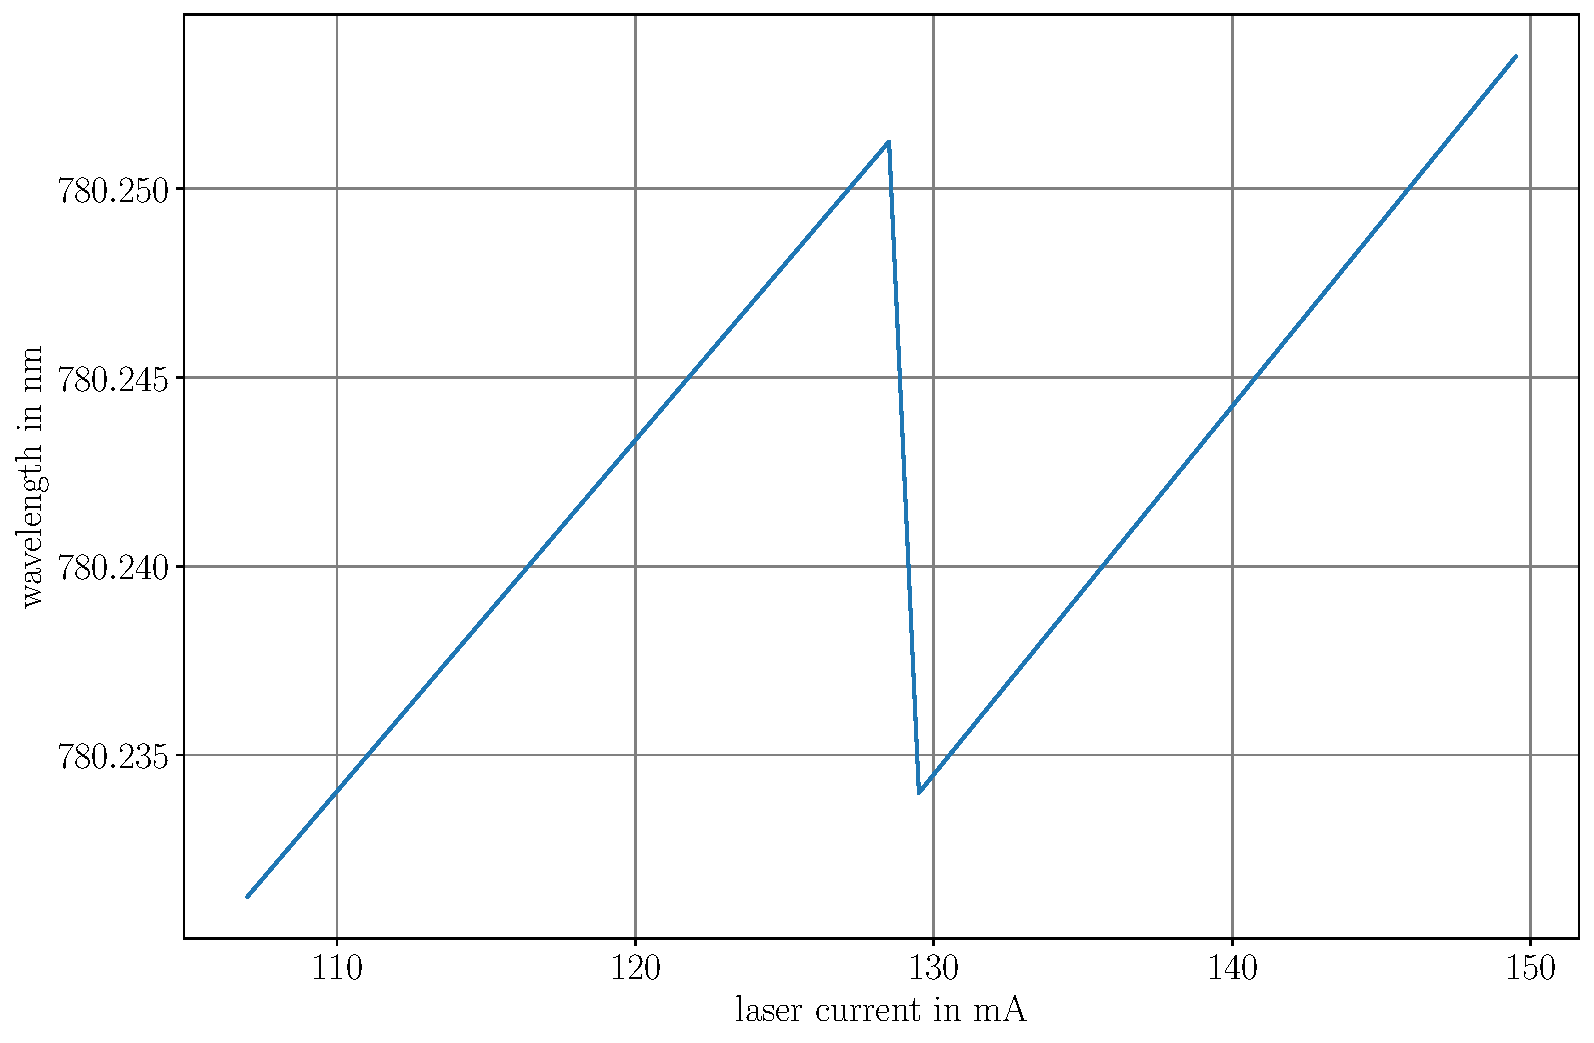
\includegraphics[scale=0.45]{Aufg-1/currentTuning.pdf}
    \captionof{figure}{cut current wavelength curve from 105 mA to 150 mA using python}
    \label{image:currentTuningCut}
\end{center}
From the csv-file we can easily find our value for the peaks of the reference beam and convert them into the corresponding wavelength. Then we compared the measured wavelength with the literature there $F$ are the quantum number of the $5^2S_{1/2}$-state.
\begin{center}
    \begin{tabular}{c | c | c c c | c c }
        \makecell{peak\\order} & \makecell{laser\\current/mA} & \makecell{wavelength\\measured/nm} & \makecell{wavelength\\literature/nm} & deviation/nm & isotope & $F$ \\
        \hline
        1 & 119.4429 & 780.243 & 780.233 & 0.010 & $^{87}Rb$ & 1 \\
        2 & 125.0267 & 780.248 & 780.238 & 0.010 & $^{85}Rb$ & 2 \\
        3 & 131.8581 & 780.236 & 780.244 & 0.008 & $^{85}Rb$ & 3 \\
        4 & 134.7829 & 780.239 & 780.246 & 0.007 & $^{87}Rb$ & 2 \\       
    \end{tabular}
    \captionof{table}{identification by intensity and order}
    \label{tab:identify}
\end{center}
Because $^{85}Rb$ have to be isotope with the highest occurrence we can clearly identify the highest peaks of the absorption spectrum as the one of $^{85}Rb$. In addition to that we can conclude that the measured data have some kind of bias, roughly 0.010 nm, in each area of the current wavelength curve of the laser.
\section{Distance between Energy Levels}
\label{sec:distance}
\subsection*{Current Wavelength Curve}
As mentioned in chapter \ref{sec:freeing} we already have transformed all data into the wavelength using the current wavelength curve. Because of that the order of the peaks has changed to 3 4 1 2. The next step is to transform the wavelength into the frequency using the formula $\nu=\frac{c}{\lambda}$, where $c$ is the speed of light in vacuum. The result can be seen in fig. \ref{image:fequency}.
\begin{center}
    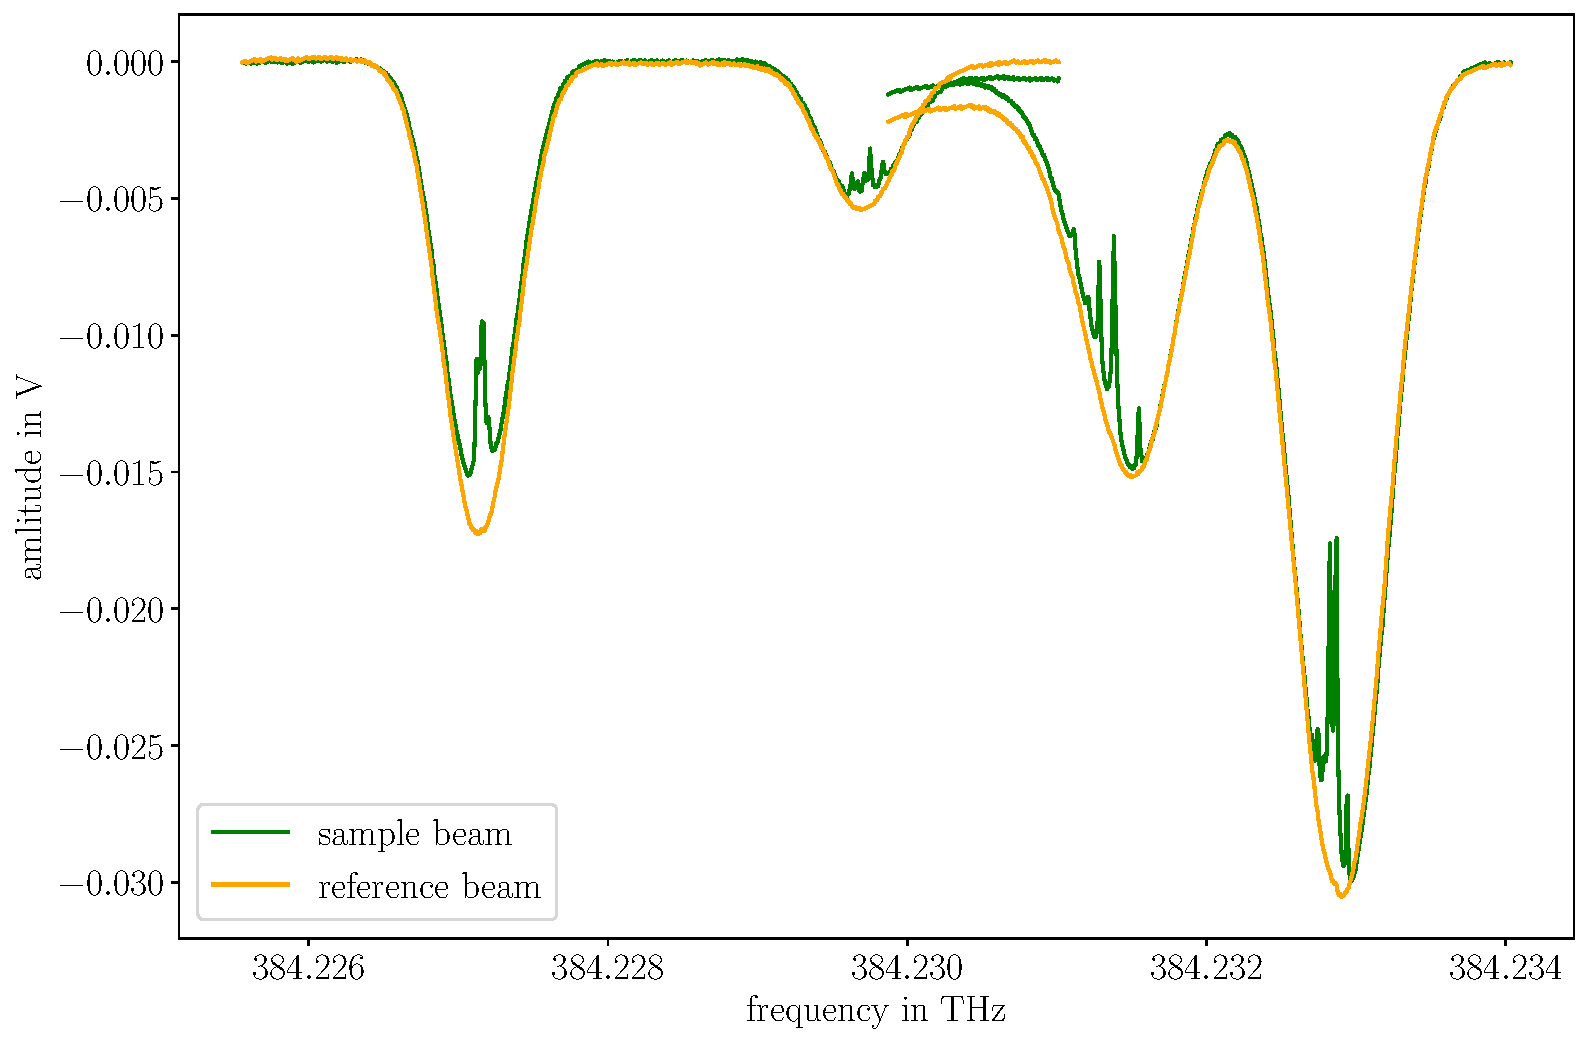
\includegraphics[scale=0.47]{Aufg-2/frequencyallPeakTemp24.pdf}
    \captionof{figure}{absorption spectrum after transformation to frequency}
    \label{image:fequency}
\end{center}
One can also see the occurrence of overlapping in fig. \ref{image:fequency} that is caused by the transformation from the laser current to the wavelength. It is possible to erase the overlapping lines from the data but for this evaluation it is necessary.
By using the same method as in chapter \ref{sec:freeing} to identify the peaks we obtain distance as followed:
\begin{center}
    \begin{tabular}{c | c}
        peak area & $d_{current}$/THz\\
        \hline
        $2 \rightarrow 1$ & 0.00256\\
        $1 \rightarrow 4$ & 0.00181\\
        $4 \rightarrow 3$ & 0.00140\\
    \end{tabular}
    \captionof{table}{distances between the energy levels using current wavelength curve}
    \label{tab:currentMethode}
\end{center}
\subsection*{Fabry-Pérot Interferometer}
To calculate the distance of the energy level we start using the function of the Fabry-Pérot interferometer and insert the measured length $d$:
\begin{gather}
    \Delta\omega_{FSR} = \frac{c}{2nd} \overset{n=1}{=} \frac{c}{2d} \overset{d=\SI{1.515}{\metre}}{=} \SI{98.9}{\mega\hertz} 
\end{gather}
In the trendfree line of the interferometer we can count from 117.0455 mA to 137.6816 mA an amount of 97 maxima peaks what gives as relation:
\begin{gather}
    \frac{97\cdot \Delta\omega_{FSR}}{\SI{137.6816}{\milli\ampere}-\SI{117.0455}{\milli\ampere}} = 0.465\frac{\si{\giga\hertz}}{\si{\milli\ampere}}
\end{gather}
This means that 1 mA correspond to \SI{0.465}{\giga\hertz}. In following we use the table \ref{tab:identify} from chapter \ref{sec:freeing} for the information of the current for each peak and take the difference of them. That gives us in comparsion with the calculated data from table \ref{tab:currentMethode}:
\begin{center}
    \begin{tabular}{c | c c c}
        peak area & difference/mA & $d_{interferometer}$/THz & $d_{current}$/THz\\
        \hline
        $1 \rightarrow 2$ & 5.5838 & 0.00260 & 0.00256\\
        $2 \rightarrow 3$ & 6.8314 & 0.00318 &   ---  \\
        $3 \rightarrow 4$ & 2.9248 & 0.00136 & 0.00140\\
    \end{tabular}
    \captionof{table}{distance between the energy levels using Fabry-Pérot interferometer and comparison to usage of current wavelength curve}
    \label{tab:interferometerMethode}
\end{center} 
In table \ref{tab:interferometerMethode} we can clearly see that both methods are equal in evaluation.
\newpage
\section{The real ratio of the rubidium isotopes}
\label{sec:ratio}
Now we calculate the ratio of each isotope by identifying the area under every peak. For that we are fitting the gaussian distribution for each peak of our data for the reference beam absorption spectrum. We take the current axis because for the ratio it does not matter which axis we use. Furthermore, we use the data that is freed from any trends (look fig. \ref{image:trendless}).Then the fitting function has the form of:
\begin{gather}
    y = a\cdot\exp(-\left(\frac{(x-b)}{\sqrt{2}c}\right)^2)
    \label{eq:gaussFit}
\end{gather}
$b$ is here the x-value of each peak that we have already obtained in table \ref{tab:identify}. We get with the curve_fit of scipy.optimize package from python:
\begin{center}
    \begin{tabular}{c | c c c}
        Peak & a/V & b/mA & c/mA\\
        \hline
        1 &  -0.00539 & 119.4429 & 0.57669\\
        2 &  -0.01742 & 125.0267 & 0.52976\\
        3 &  -0.03085 & 131.8581 & 0.62443\\
        4 &  -0.01462 & 134.7829 & 0.74425\\
    \end{tabular}
    \captionof{table}{Fitting data for each peak}
\end{center}
In figure \ref{image:gaussFit} is shown how each gaussian fit looks for each peak.\\
With the parameter we calculated above we are now able to determine the area under each curve of each peak with the following relation:
\begin{gather}
    \int^{\infty}_{-\infty}\exp(-k(x-\mu)^2)\,dx = \sqrt{\frac{\pi}{k}} \xrightarrow{\mu = b,~k = \frac{1}{2c^2}}\int^{\infty}_{-\infty}a\cdot\exp(-\left(\frac{(x-b)}{\sqrt{2}c}\right)^2) = a \sqrt{2\pi c^2}
\end{gather}
This expression gives us then the area as follows:
\begin{center}
    \begin{tabular}{c | c | c}
        Peak & isotope & area/$1\cdot 10^{-6}$ W\\
        \hline
        1 & $^{87}Rb$ &  -7.79 \\
        2 & $^{85}Rb$ & -23.13 \\
        3 & $^{85}Rb$ & -48.29 \\
        4 & $^{87}Rb$ & -27.27 \\
    \end{tabular}
\end{center}
The area under the peaks is proportional to the amount of atoms of each isotope in the gas what gives us:
\begin{gather}
    ^{85}Rb = \frac{23.13+48.29}{7.79+23.13+48.29+27.27} = 0.671 \Rightarrow  {^{87}Rb} = 0.329
\end{gather}
Meaning that in our probe there is \SI{67.1}{\percent} $^{85}Rb$ and \SI{32.9}{\percent} $^{87}Rb$ which compared to the literature (\SI{72.2}{\percent} $^{85}Rb$ and \SI{27.8}{\percent} $^{87}Rb$) shows that the assumption from chapter \ref{sec:freeing} to take the intensity into account was correct.
\begin{center}
    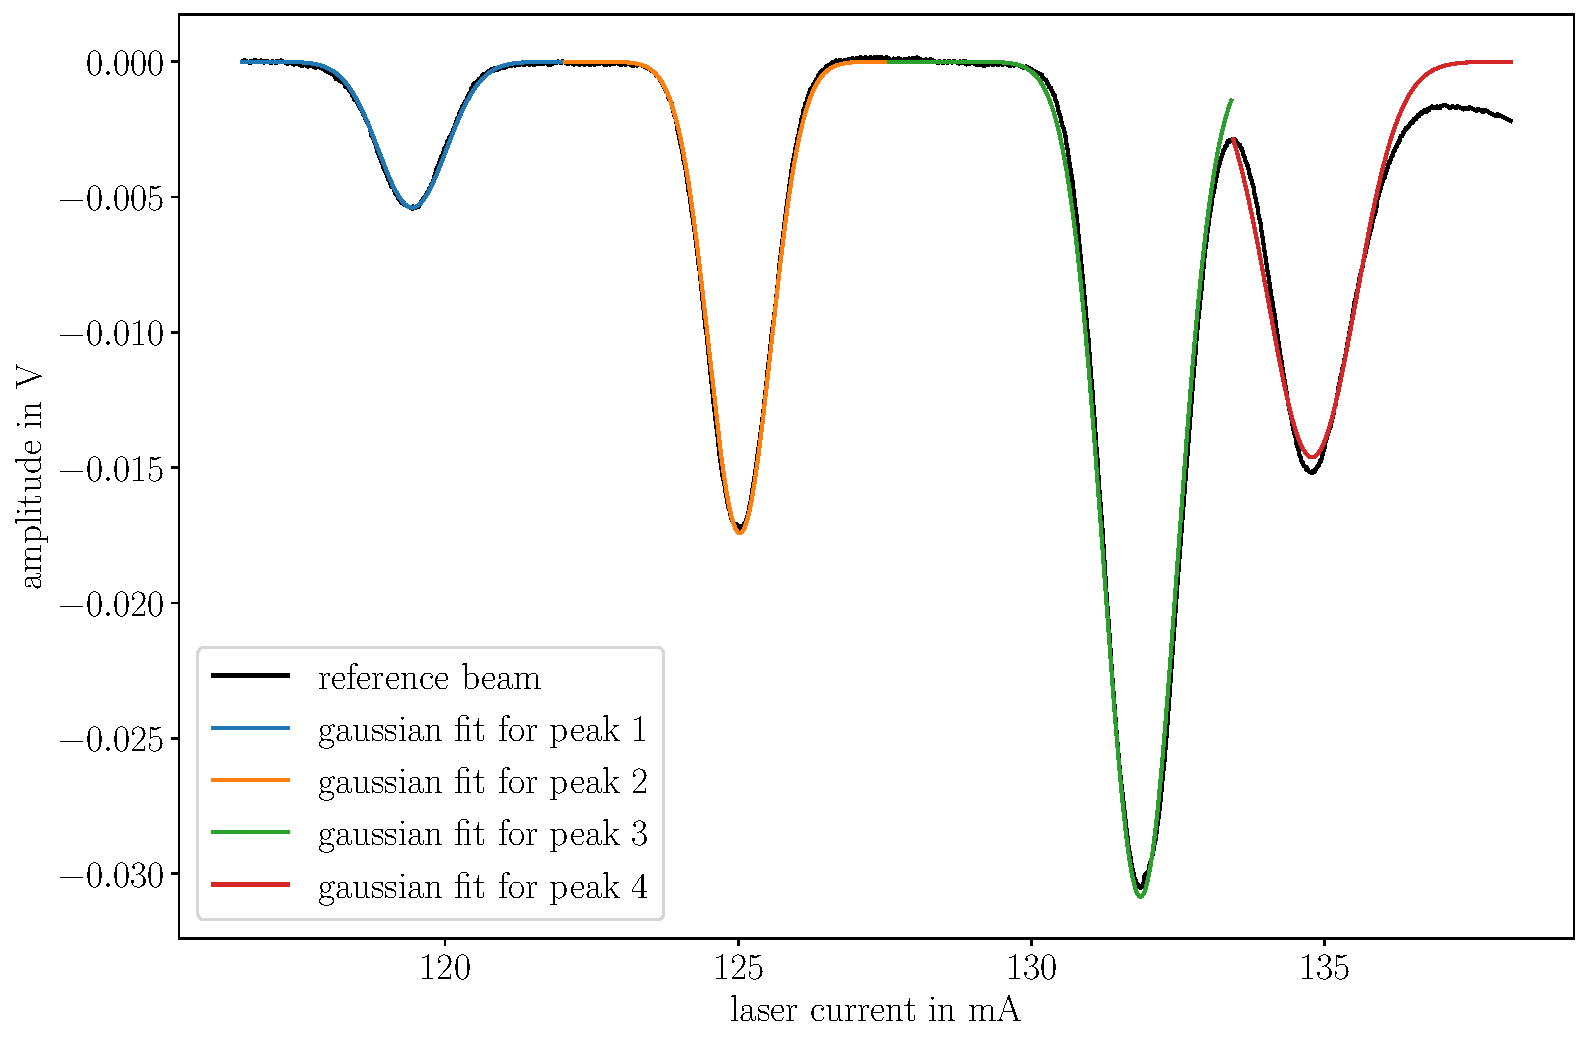
\includegraphics[scale=0.72, angle = 90]{Aufg-3/gaussFit.pdf}
    \captionof{figure}{gaussian fit for each Peak of the reference beam spectrum}
    \label{image:gaussFit}
\end{center}
\section{Hyperfine Dips}
\label{sec:hyperfine}
Firstly we want to show all absorption dips separately starting with peak 1 and ending with peak 4.
\begin{center}
    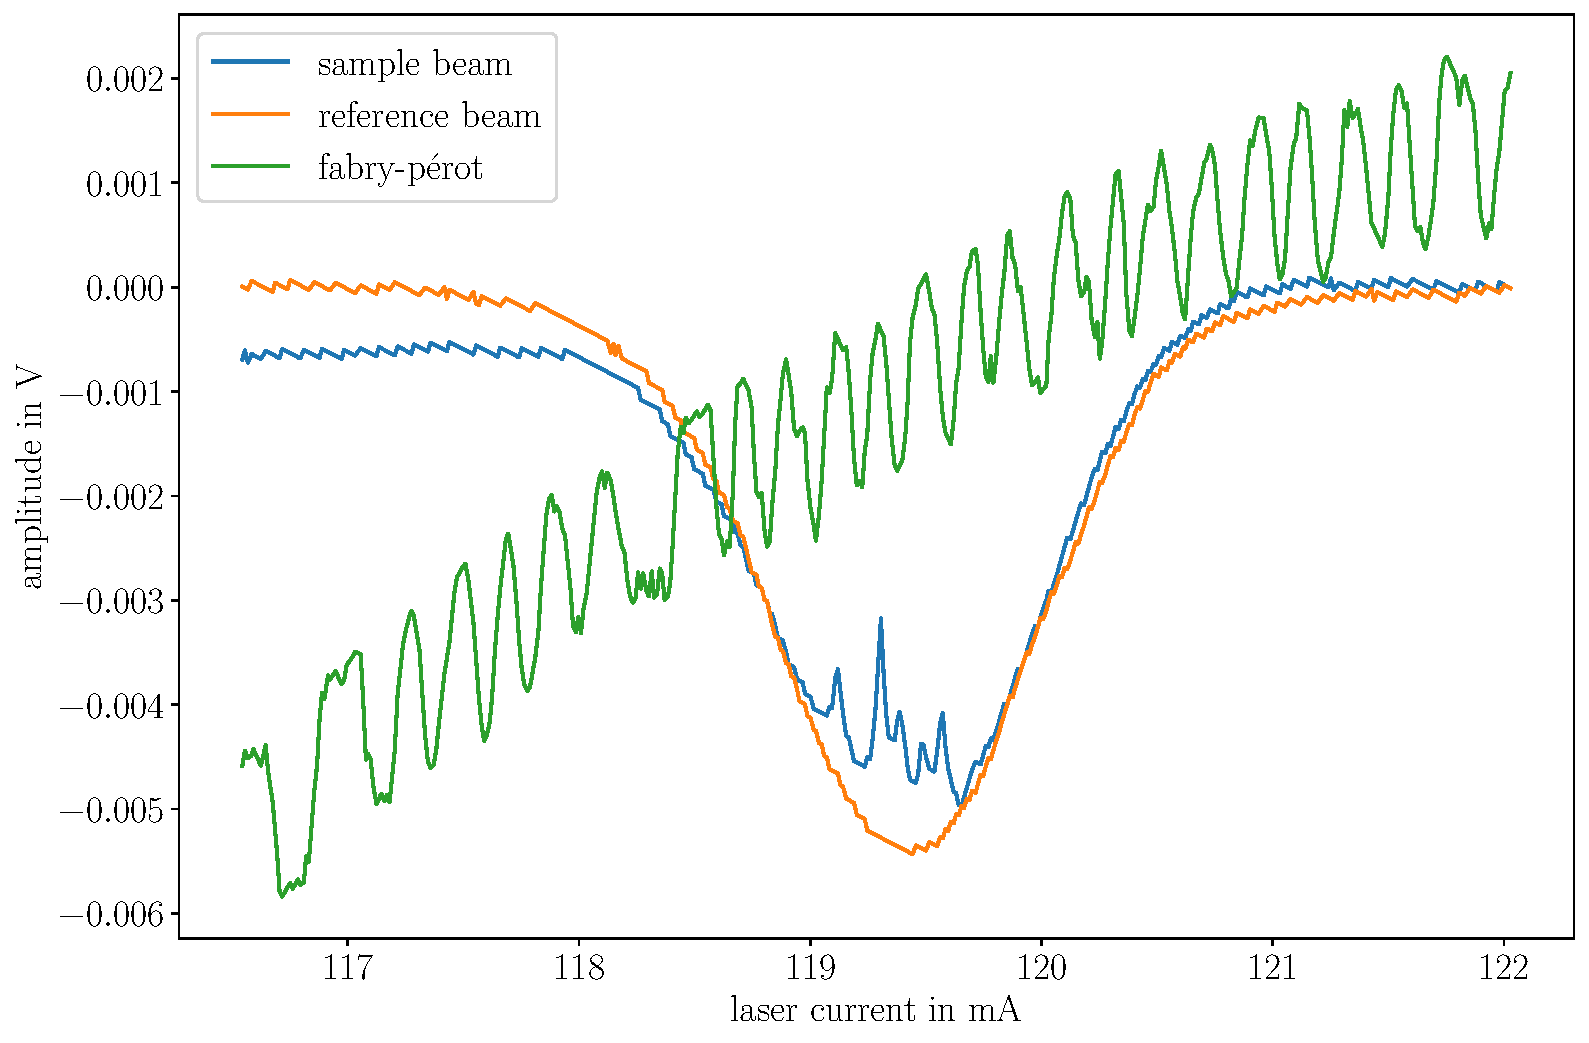
\includegraphics[scale=0.47]{Aufg-4/hyperfine1.pdf}
    \captionof{figure}{absorption spectrum of peak number 1}
    \label{image:peak1}
\end{center}
\begin{center}
    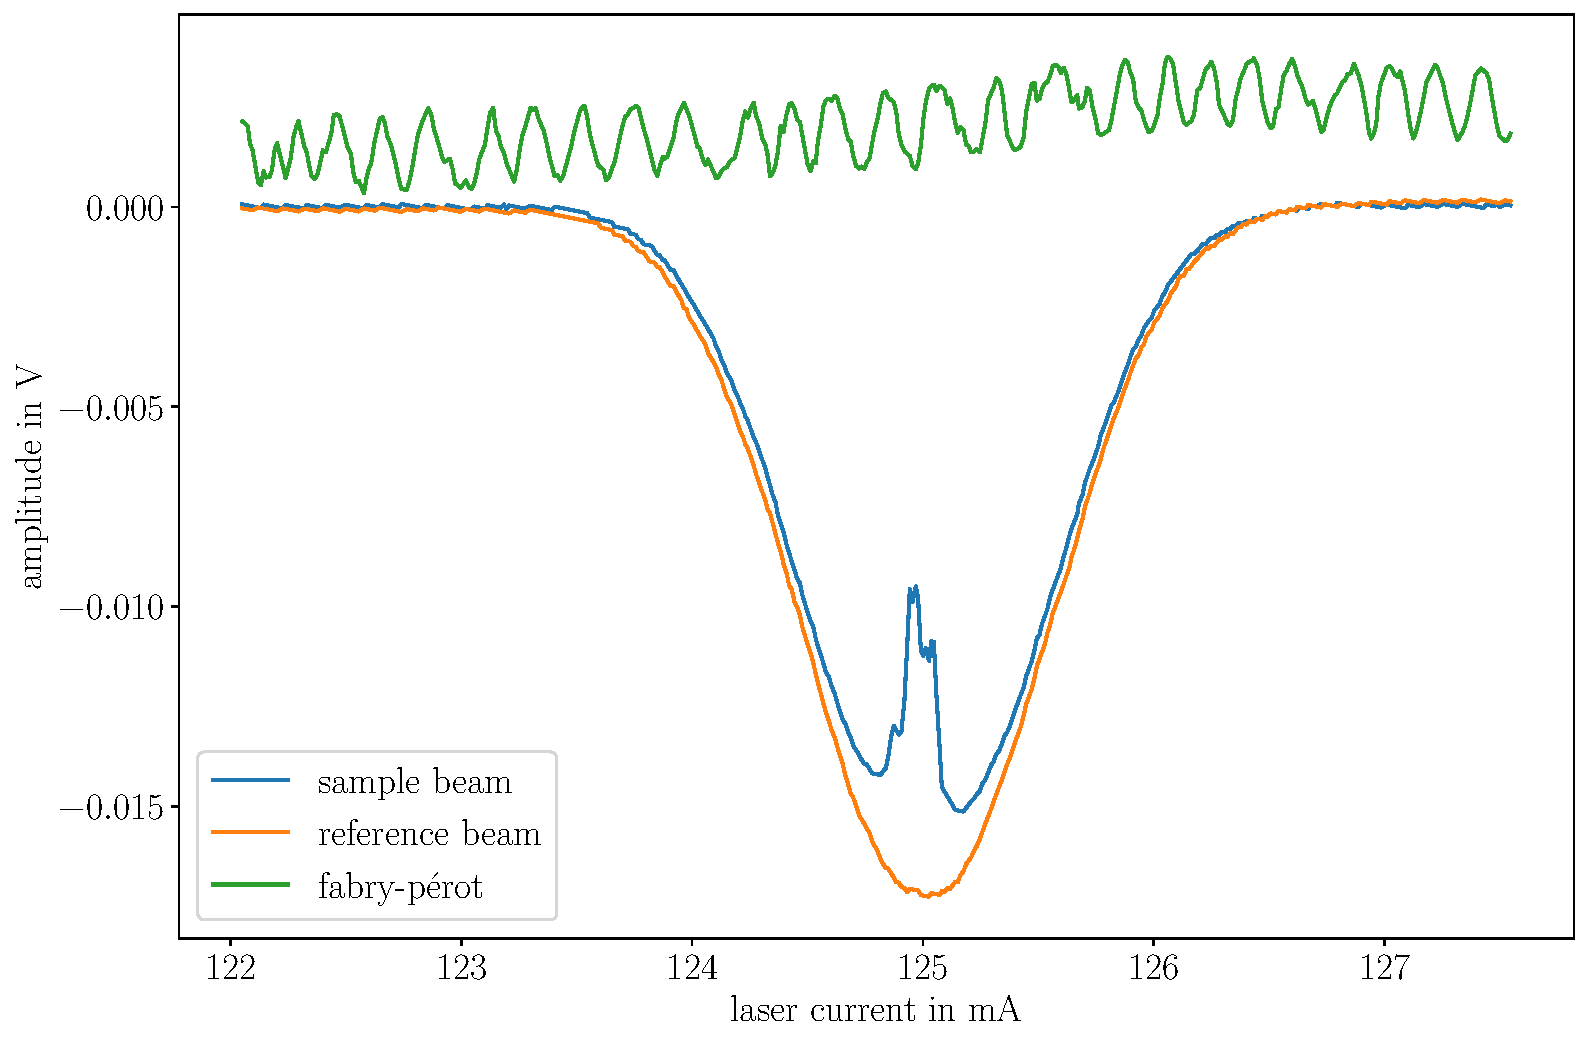
\includegraphics[scale=0.47]{Aufg-4/hyperfine2.pdf}
    \captionof{figure}{absorption spectrum of peak number 2}
    \label{image:peak2}
\end{center}
\begin{center}
    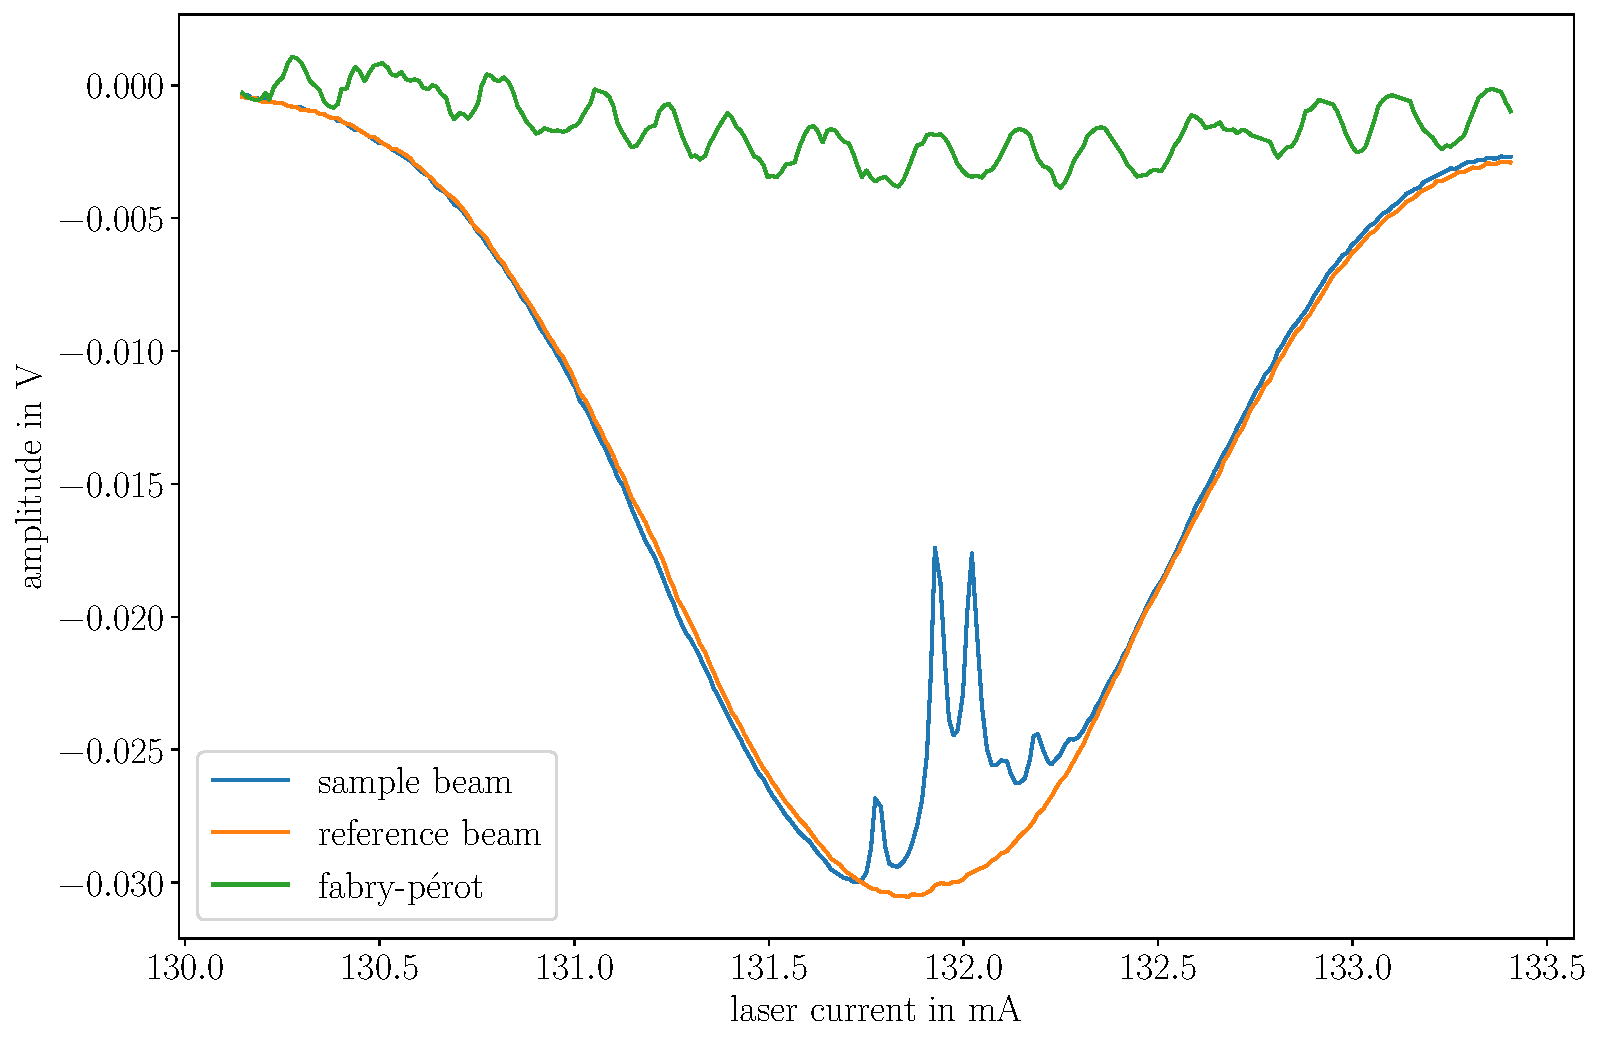
\includegraphics[scale=0.47]{Aufg-4/hyperfine3.pdf}
    \captionof{figure}{absorption spectrum of peak number 3}
    \label{image:peak3}
\end{center}
\begin{center}
    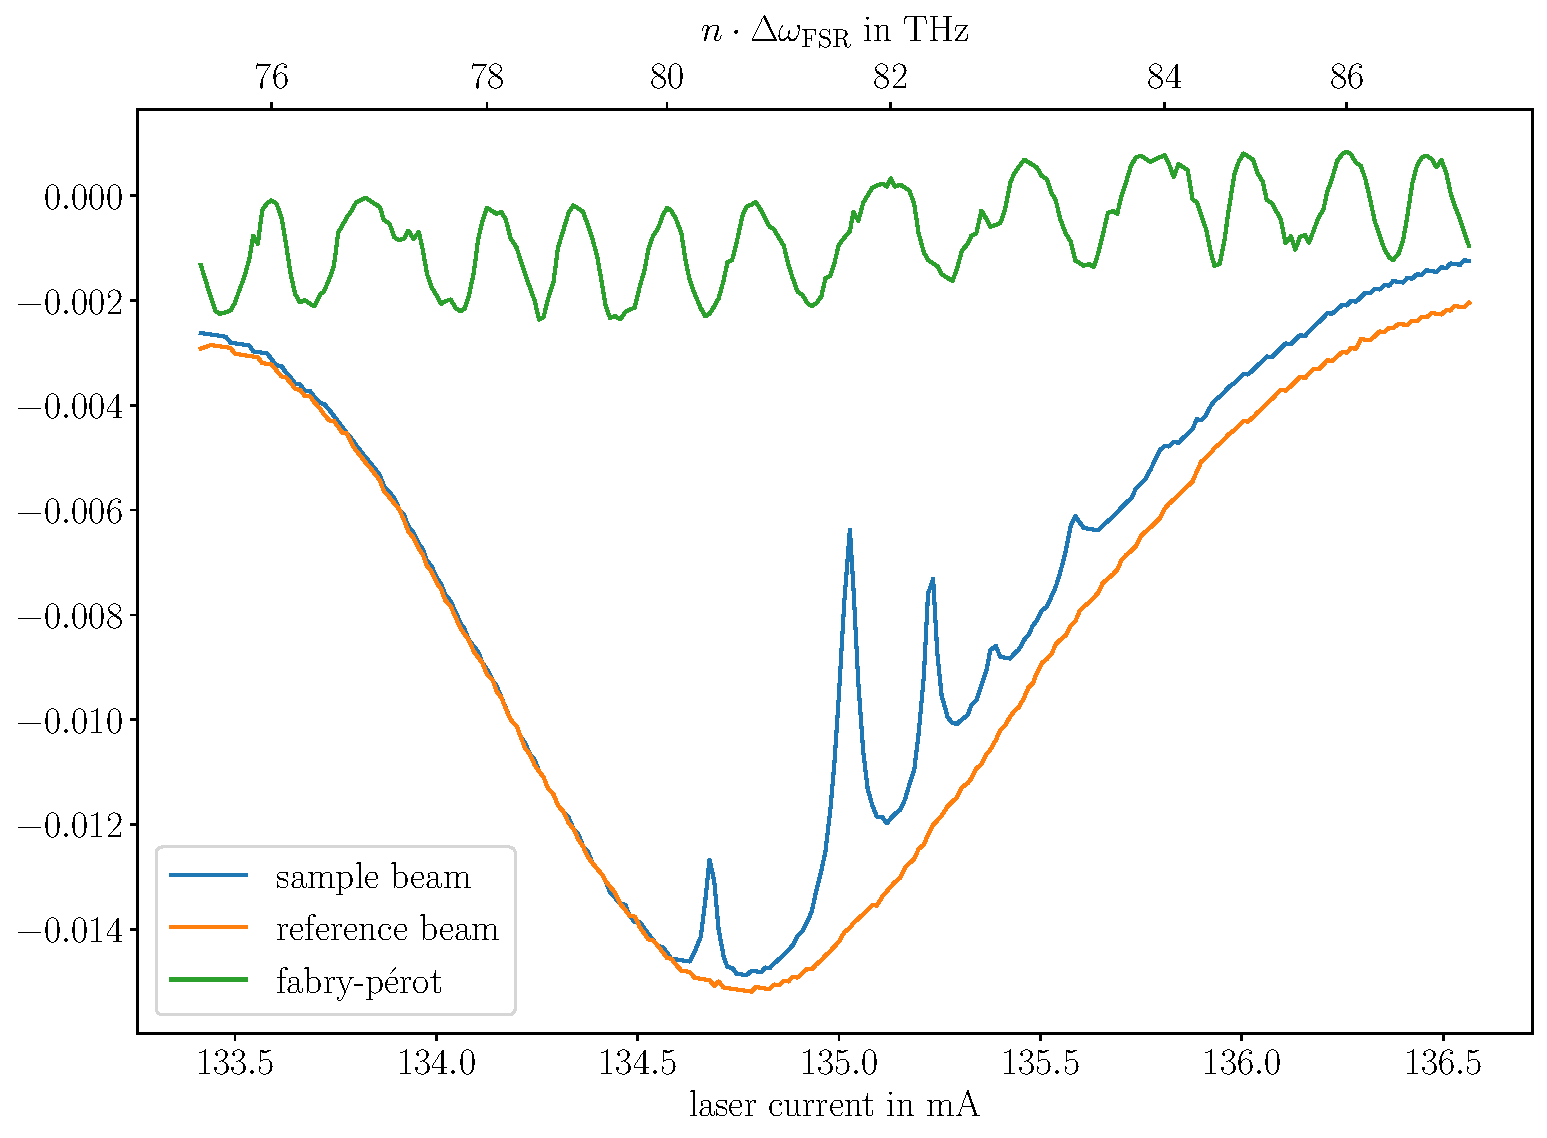
\includegraphics[scale=0.47]{Aufg-4/hyperfine4.pdf}
    \captionof{figure}{absorption spectrum of peak number 4}
    \label{image:peak4}
\end{center}
\newpage
It was chosen to use the peak number 3 because there are the hyperfine dips clearly visible. Its the isotope $^{85}Rb$. For the upcuming calculation we will use the measured data of peak 3 only because of that we have had an offset in our data from $z_{off}=\SI{0.072}{\volt}$ and have to transform the laser current again like in chapter \ref{sec:freeing} into wavelength and frequency.
The fit of the Lorentz curve (lorentzian) was achieved with the function:
\begin{gather}
    y = \frac{a c^2}{(x-b)^2+c^2} - d
\end{gather}
By observing the formula of the fit it gets clear that $a$ is nothing else as the laser current value and $b$ the amplitude of each hyperfine dip peak. From that conclusion we get for the hyperfine peaks numbered from left to right:
\begin{center}
    \begin{tabular}{c | c c c c c c}
        \makecell{hyperfine\\peak} &\makecell{$a$/mA} & $a$/nm &  $a$/THz &  $b$/V & $c$/mA & $d$/V \\
        \hline
        1   &   131.8489  &  780.236290  &  384.232907   &  -0.0269 & -0.0266 & -0.032\\
        2   &   132.0006  &  780.236438  &  384.232834   &  -0.0169 & -0.0285 & -0.032\\
        3   &   132.0778  &  780.236513  &  384.232797   &  -0.0177 & -0.0325 & -0.032\\
        4   &   132.1607  &  780.236594  &  384.232757   &  -0.0254 & -0.0680 & -0.032\\
        5   &   132.2349  &  780.236667  &  384.232722   &  -0.0243 & -0.0613 & -0.032\\
        \end{tabular}
        \captionof{table}{fitting data for each hyperfine dip}
        \label{tab:lorFit}
\end{center}
Furthermore the lorentzian fit for each dip can be seen in fig. \ref{image:lorFit}.\\
It is clear that there are more dips than possible hyperfine transition. In case of $^{85}Rb$ each dip represents a transition from energy levels $F=3$ of the state $5^2S_{1/2}$ to a different energy level of the $5^2P_{3/2}$ state with quantum number $F'$, in short: $F=3\rightarrow F'$. With the selection rule of the hyperfine transition ($\Delta F = 0,\pm1$) we obtain that there should be only three dips visible ($F'=2,3,4$) the remaining dips come from cross over resonances.
For Comparison with the literature we calculate the distance between the dips using table \ref{tab:lorFit} and obtain:
\begin{center}
    \begin{tabular}{c | c c | c c}
        \makecell{dip area} & \makecell{distance\\measured/MHz} & \makecell{distance\\literature/MHz} & \makecell{transition\\ $F'_1\leftrightarrow F'_2$} \\
        \hline
        $1\rightarrow 2$ & 73.00 & 63.38 & $2\leftrightarrow 3$ \\
        $2\rightarrow 5$ & 114.00 & 120.99 & $3\leftrightarrow 4$\\
    \end{tabular}
    \captionof{table}{distance between the selected dips}
\end{center}
The Comparison with the literature shows us that indeed the peek 3 should be $^{85}Rb$ as we assumed in chapter \ref{sec:freeing} and \ref{sec:ratio}. The difference between literature and measurement could have the same cause as the difference in chapter \ref{sec:freeing}.
\newpage
\begin{center}
    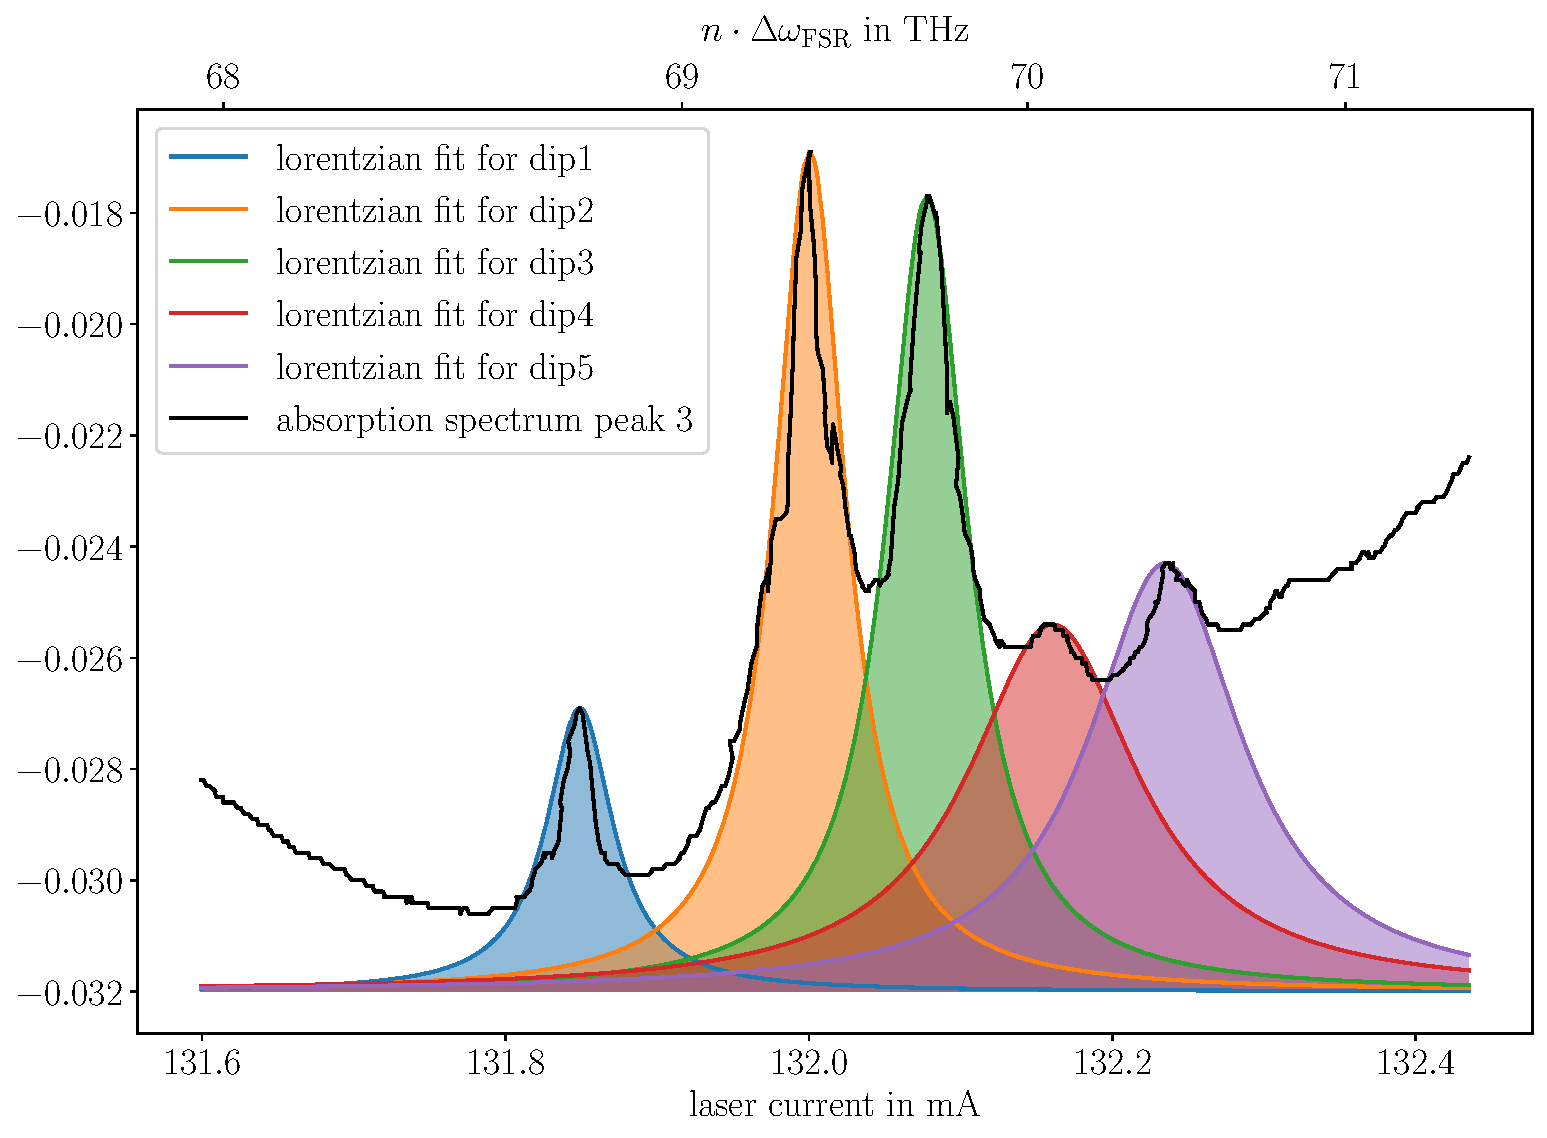
\includegraphics[scale=0.72, angle = 90]{Aufg-4/hyperfinePeak3.pdf}
    \captionof{figure}{lorentzian fit for each dip of peak 3}
    \label{image:lorFit}
\end{center}

%$1\rightarrow 2$ & 73.0 & & \\
%        $2\rightarrow 3$ & 37.0 & & \\
%        $3\rightarrow 4$ & 40.0 & & \\
%        $4\rightarrow 5$ & 37.0 & & \\
\section{Hyperfine constant}
In the following we use the equation \ref{eq:HFS} to calculate the hyperfine constants.
\begin{align}
    \label{eq:HFS}
    \Delta E_{HFS} = \frac{a}{2} [F(F+1) - J(J+1) - I(I+1)]
\end{align}
We know the Energy difference and the Quantum numbers of the transitions from table \ref{tab:disDip}. So we can rewrite the equation: 
\begin{align}
    a = \frac{2(\Delta E)}{F_2(F_2+1)-F_1(F_1+1)} \qquad \text{mit} \quad \Delta E = h \cdot \Delta \nu
\end{align}
After we put in the values we get the following results: 
\begin{table}[h]
    \centering
\begin{tabular}{c|c|c}
    transition & a in $10^{-26}$ J & literature: a in $10^{-26}$ J \\
    \hline
    $2\leftrightarrow 3$ & 1.612 & 1.400\\
    $3\leftrightarrow 4$ & 1.888 & 1.840
\end{tabular}
\caption{hyperfine constants}
\end{table} \\
The literature value of $a$ is computed by the literature value of $\Delta \nu$ from table \ref{tab:disDip}. The difference of one value cloud have the same problem as mentioned in chapter \ref{sec:hyperfine}. 

% etc.

    % 5.Chapter Closure
    % 5. Closure

\chapter{Closure}
\label{chap:close}


% Text

    % Appendix
    %% Appendix

\appendix

% Text

% Charlotte Geiger - Manuel Lippert - Leonard Schatt
% Physikalisches Praktikum

% Anhang A

\chapter{Append A}
\label{chap:anhangA}

\section{Teilanhang X}


    % Literatur
    \bibliographystyle{Auswertung.bst}
    \bibliography{Auswertung.bib}
    
\end{document}